\documentclass[12pt]{article}
\usepackage{../../preamble3}
%\pagenumbering{gobble}
\title{MathCounts Chapter Invitational February 2021 \\ Target Round}
\author{Patrick \& James Toche}
\date{Revised:~\today}

\begin{document}
\maketitle
\begin{minipage}{\textwidth}
\begin{abstract}\setlength{\parindent}{0pt}%
Notes on Target Round of MathCounts Invitational Competition, February 2021. 
Questions are from MathCounts Foundation (\url{https://www.mathcounts.org/}). Copyright restrictions may apply. Written for personal use. 
Please report typos and errors over at \url{https://github.com/ptoche/Math/tree/master/mathcounts}. 
\end{abstract}
\end{minipage}

\thispagestyle{empty}
\clearpage
\addtocounter{page}{-1}

\section*{Target Round}


%%%%%%%%%%%%%%%%%%%%%%%%%%%%%%%%%%%%%%%%%%%%%%%%%%%%%%%%%%%%%%%%%%%%%%%%
\subsection*{1.}
Max is buying hot dogs and buns for dinner. If hot dogs are sold in packages of six and buns are sold in packages of eight, what is the least positive number of hot dogs that Max must buy so that he can purchase exactly the same number of buns? 

\fbox{\phantom{ANSWER}}~hot dogs

\begin{answer}
The least common multiple of $6$ and $8$ can be found with one of these approaches: 
\begin{enumerate}
\item list multiples of $6$ until one of them is a multiple of $8$.
\item list multiples of $8$ until one of them is a multiple of $6$.
\end{enumerate}
The second approach would be a little quicker. We have $8$, $16$, $24$, stop.
\begin{empheq}[box={\mathbox[colback=white]}]{equation*}
    24 ~\text{hot dogs}
\end{empheq} 
\end{answer}
%%%%%%%%%%%%%%%%%%%%%%%%%%%%%%%%%%%%%%%%%%%%%%%%%%%%%%%%%%%%%%%%%%%%%%%%


%%%%%%%%%%%%%%%%%%%%%%%%%%%%%%%%%%%%%%%%%%%%%%%%%%%%%%%%%%%%%%%%%%%%%%%%
\subsection*{2.}
The square card shown in Figure~A, with area $16$ units$^2$, is folded twice along the dashed lines to get the square shown in Figure~B. Then, scissors are used to cut through the folded square, and one-fourth of the folded card, shown shaded in Figure~C, is removed. When unfolded, what is the area of what remains of the card after the removal? 

\begin{center}
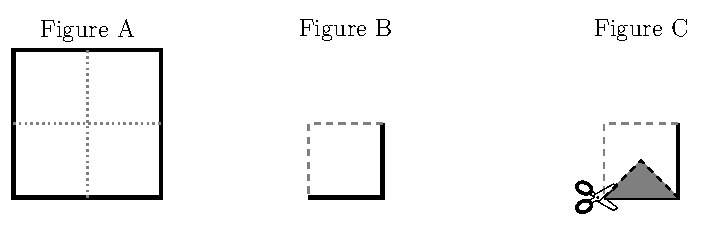
\includegraphics[height=6cm]{target-02-figure}
\end{center}

\nopagebreak

\fbox{\phantom{ANSWER}}~units$^2$

\begin{answer}
The area removed by one triangular cut is equal to one-fourth of one-fourth of the large square in Figure~A. Because of the folding, there are four such triangular cuts, so that the total area removed is one-fourth of the area of the large square, or $16/4=4$. The area of what remains is therefore $16-4=12$. 
\begin{empheq}[box={\mathbox[colback=white]}]{equation*}
    12 ~\text{units}^2
\end{empheq} 
\end{answer}
%%%%%%%%%%%%%%%%%%%%%%%%%%%%%%%%%%%%%%%%%%%%%%%%%%%%%%%%%%%%%%%%%%%%%%%%


%%%%%%%%%%%%%%%%%%%%%%%%%%%%%%%%%%%%%%%%%%%%%%%%%%%%%%%%%%%%%%%%%%%%%%%%
\subsection*{3.}
Cindy has been given four chores to complete today: vacuum, mop, dust and laundry. Because Cindy finds doing laundry especially unpleasant, she wants to do that chore last. Given this, in how many different orders can Cindy complete her chores? 

\nopagebreak

\fbox{\phantom{ANSWER}}~orders

\begin{answer}
One of the $4$ objects has its position predetermined (laundry), so that we are looking for the number of ways to permute $3$ objects.
\begin{align*}
3! = 3 \times 2 = 6
\end{align*}
\begin{empheq}[box={\mathbox[colback=white]}]{equation*}
    6 ~\text{orders}
\end{empheq} 
\end{answer}
%%%%%%%%%%%%%%%%%%%%%%%%%%%%%%%%%%%%%%%%%%%%%%%%%%%%%%%%%%%%%%%%%%%%%%%%

\iftoggle{showAnswers}{\newpage}

%%%%%%%%%%%%%%%%%%%%%%%%%%%%%%%%%%%%%%%%%%%%%%%%%%%%%%%%%%%%%%%%%%%%%%%%
\subsection*{4.}
In the dice game Zero, a player rolls six standard six-sided dice and then scores points for certain combinations, as shown in the table. A die cannot be used in more than one combination. For example, a player who rolls $1$~$5$~$6$~$4$~$4$~$6$ scores $50$ points, while a player who rolls $1$~$4$~$4$~$4$~$1$~$4$ scores $250$ points. What is the probability that a player scores $0$ points on a roll? Express your answer as a common fraction. 

\begin{center}
  \rowcolors{1}{white}{gray!20}
\begin{tabular}{L{6cm}R{3cm}} 
\toprule
  Player's Roll & Points Scored \\
\midrule
  Three of a kind (ex. $2$~$2$~$2$~$4$~$6$~$3$) & 100 \\
  Four of a kind                                & 200 \\
  Five of a kind                                & 400 \\
  Six of a kind                                 & 900 \\
  Three pairs (ex. $2$~$2$~$3$~$3$~$4$~$4$)     & 200 \\
  Six distinct (ex. $1$~$2$~$3$~$4$~$5$~$6$)    & 300 \\
  The number $1$                                &  25 \\
  The number $5$                                &  25 \\
\bottomrule
\end{tabular}
\end{center}

\nopagebreak

\begin{minipage}[b]{\linewidth}
\fbox{\phantom{ANSWER}}\\
\mbox{---------------}\\
\fbox{\phantom{ANSWER}}
\end{minipage}

\begin{answer}
The configurations that yield no points are $2$~$3$~$4$~$6$ with two numbers repeated but no triple. The number of ways to choose $2$ objects from $6$ is 
\begin{align*}
\comb{2}{6} = \frac{6!}{2!(6-2)!} = \frac{6 \times 5}{2} = 15
\end{align*}
To properly calculate the probability, we also need to take into account permutations of these six rolls ($6!$).
The number of ways to roll six six-sided dice is $6^6$. 
Thus, the probability is the ratio of these:
\begin{align*}
\frac{15 \times 6!}{6^6} 
  = \frac{5}{216}
\end{align*}
\begin{empheq}[box={\mathbox[colback=white]}]{equation*}
    \frac{5}{216}
\end{empheq} 
\end{answer}
%%%%%%%%%%%%%%%%%%%%%%%%%%%%%%%%%%%%%%%%%%%%%%%%%%%%%%%%%%%%%%%%%%%%%%%%

\iftoggle{showAnswers}{\newpage}

%%%%%%%%%%%%%%%%%%%%%%%%%%%%%%%%%%%%%%%%%%%%%%%%%%%%%%%%%%%%%%%%%%%%%%%%
\subsection*{5.}
A U.S. quarter is $0.069$ inches thick. Clayton Kershaw earned $33$ million dollars for the $2017$ Major League Baseball season. If Kershaw received his entire $2017$ salary in the form of a single stack of quarters, what would be the height of the stack, in miles? There are $5280$ feet in a mile. Express your answer as a decimal to the nearest hundredth. 

\nopagebreak

\fbox{\phantom{ANSWER}}~units$^2$

\begin{answer}
A dollar in quarters is 
\begin{align*}
4 \times 0.069 = 0.276 ~\text{inches}
\end{align*}
$33$ million of those is 
\begin{align*}
33 \times 0.276 = 9,108,000 ~\text{inches}
\end{align*}
Converted to feet:
\begin{align*}
9,108,000~\text{inches} \times \frac{1~\text{foot}}{12~\text{inches}} = 759,000~\text{feet}
\end{align*}
Converted to miles:
\begin{align*}
759,000~\text{feet} \times \frac{1~\text{mile}}{5280~\text{feet}}
 = 143.75~\text{miles} 
\end{align*}
\begin{empheq}[box={\mathbox[colback=white]}]{equation*}
    143.75~\text{miles} 
\end{empheq} 
\end{answer}
%%%%%%%%%%%%%%%%%%%%%%%%%%%%%%%%%%%%%%%%%%%%%%%%%%%%%%%%%%%%%%%%%%%%%%%%

\iftoggle{showAnswers}{\newpage}

%%%%%%%%%%%%%%%%%%%%%%%%%%%%%%%%%%%%%%%%%%%%%%%%%%%%%%%%%%%%%%%%%%%%%%%%
\subsection*{6.}
In rectangle ABCD the length of side AB is less than the length of side BC. When diagonal AC is drawn, and a line segment from vertex B to diagonal $AC$ is drawn so that the segment meets AC at a right angle, rectangle ABCD is divided into three regions whose areas form an arithmetic progression. The ratio AB{:}BC, expressed as a common fraction in simplest radical form is $\dfrac{\sqrt{a}}{b}$. What is the value of $ab$? 

\nopagebreak

\fbox{\phantom{ANSWER}}

\begin{answer}
\begin{center}
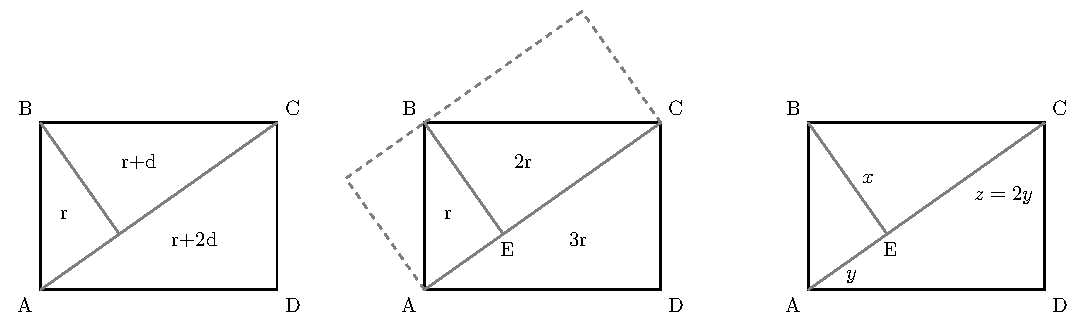
\includegraphics[width=\linewidth]{target-06-figure}
\end{center}
The rectangle is divided into three regions with the following property:
\begin{align*}
r + 2d = 2r + d 
\Rightarrow r = d
\end{align*}
where $r$ denotes the area (region) of the smaller triangle and $d$ the increment (difference) in the arithmetic progression. It follows that the areas are given by $r$, $2r$, $3r$. The progression is thus both geometric and arithmetic! The geometry of the problem yields a straightforward solution. The ratio of the areas of triangle BEA and BEC is $1{:}2$ and the same is obviously true of the rectangles marked by the dashed lines (the area of each rectangle is twice the area of the triangle). These rectangles have diagonals BA and BC. Since the areas of the rectangles are in the ratio $1{:}2$, the squares of their diagonals are also in that ratio, that is
\begin{align*}
\frac{\text{AB}^2}{\text{BC}^2} = \frac{1}{2}
\end{align*}
which yields the ratio: 
\begin{align*}
\frac{\text{AB}}{\text{BC}} = \frac{1}{\sqrt{2}}
  = \frac{\sqrt{2}}{2}
\end{align*}
The values of $a$ and $b$ follows immediately: 
\begin{empheq}[box={\mathbox[colback=white]}]{equation*}
    \frac{\sqrt{a}}{b} = \frac{\sqrt{2}}{2}
    \Rightarrow ab = 4
\end{empheq}
A less inspired solution involves calculating areas and manipulating expressions. Denote E the intersection of AC and the perpendicular line segment, denote $x$ the distance BE, $y$ the distance AE, and $z$ the distance CE. From the area triangle AEB, we have
\begin{align*}
xy & = 2r \\
xz & = 4r
\end{align*}
implying $z=2y$. In words, the perpendicular segment cuts the diagonal at the one-third point. Applying the Pythagoras theorem to segments AB and BC yields:
\begin{align*}
\frac{\text{AB}^2}{\text{BC}^2} 
  = \frac{x^2 + y^2}{x^2 + z^2}
  = \frac{x^2 + y^2}{x^2 + (2y)^2}
  = \frac{x^2 + 4y^2 - 3y^2}{x^2 + 4y^2}
  = 1 - \frac{3y^2}{x^2 + 4y^2}
  = 1 - \frac{3}{(x/y)^2 + 4}
\end{align*}
In addition, setting the area of rectangle ABCD to the sum of the areas of triangle BEA and triangle BEC yields:
\begin{align*}
\sqrt{x^2+y^2} \times \sqrt{x^2+4y^2} = xy + 2xy
\end{align*}
Squaring both sides of the equality and distributing the product:
\begin{align*}
(x^2 + y^2) (x^2 + 4y^2) & = (3xy)^2 \\
x^4 + 4x^2y^2 + x^2y^2 + 4y^4 & = 9x^2y^2 \\
x^4 - 4x^2y^2 + 4y^4 & = 0 \\
(x/y)^4 - 4(x/y)^2 + 4 & = 0 
\end{align*}
This is a quadratic equation in $(x/y)^2$. To see this, let $u=x/y$
\begin{align*}
u^2 - 4u + 4 & = 0 \\
(u - 2)^2 & = 0
\end{align*}
and therefore
\begin{align*}
(x/y)^2 = 2
\end{align*}
Plugging that back in the expression for the ratio, we recover the earlier result:
\begin{align*}
\left(\frac{\text{AB}}{\text{BC}}\right)^2
  = 1 - \frac{3}{2 + 4} = \frac{1}{2}
\end{align*} 
These manipulations are prone to errors, especially under time constraints, so the more intuitive approach is clearly superior. 
\end{answer}
%%%%%%%%%%%%%%%%%%%%%%%%%%%%%%%%%%%%%%%%%%%%%%%%%%%%%%%%%%%%%%%%%%%%%%%%

\iftoggle{showAnswers}{\newpage}

%%%%%%%%%%%%%%%%%%%%%%%%%%%%%%%%%%%%%%%%%%%%%%%%%%%%%%%%%%%%%%%%%%%%%%%%
\subsection*{7.}
If C is the temperature in degrees Celsius, the temperature in degrees Farenheit is given by the formula $\text{F}=\dfrac{9}{5}\text{C}+32$. On a cold winter day, the temperature in degrees Farenheit is the additive inverse of the temperature in degrees Celsius. What is the temperature in degrees Celsius? Express your answer as a decimal to the nearest tenth. 

\nopagebreak

\fbox{\phantom{ANSWER}}~$^{\circ}$C

\begin{answer}
The main difficulty here is knowing that the ``additive inverse'' of $x$ is the number $y$ such that $x+y=0$, in other words the additive inverse of $x$ is $-x$, its ``opposite.'' The verbal statement yields a system of two equations in two unknowns:
\begin{align*}
\text{F} & = \dfrac{9}{5}\text{C} + 32 \\
\text{F} & = -\text{C}
\end{align*}
which may be solved by substitution:
\begin{align*}
-\text{C} = \dfrac{9}{5}\text{C} + 32 
\Rightarrow
\left(\frac{9}{5}+1\right) \text{C} 
          = -32 
\Rightarrow
 \text{C} = -32 \times \frac{5}{14} 
          \approx -11.429
\end{align*}
\begin{empheq}[box={\mathbox[colback=white]}]{equation*}
    -11.4~^{\circ}\text{C}
\end{empheq} 
\end{answer}
%%%%%%%%%%%%%%%%%%%%%%%%%%%%%%%%%%%%%%%%%%%%%%%%%%%%%%%%%%%%%%%%%%%%%%%%

\iftoggle{showAnswers}{\newpage}

%%%%%%%%%%%%%%%%%%%%%%%%%%%%%%%%%%%%%%%%%%%%%%%%%%%%%%%%%%%%%%%%%%%%%%%%
\subsection*{8.}
How many ways are there to color the $4 \times 4$ grid shown, so that each unit square is red, blue, green, or yellow, and so that each square is the same color as exactly two of the squares that share a side with it?

\begin{center}
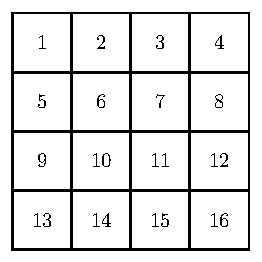
\includegraphics[height=4cm]{target-08-figure-A}
\end{center}

\nopagebreak

\fbox{\phantom{ANSWER}}~ways

\begin{answer}
Let A, B, C, D denote the four possible color choices. Here is one way to color the grid:
\begin{center}
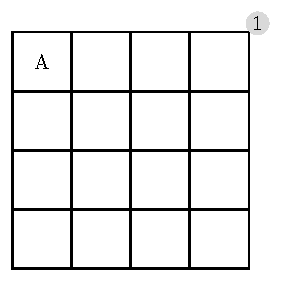
\includegraphics[width=0.3\linewidth,page=1]{target-08-figure-B}
\includegraphics[width=0.3\linewidth,page=2]{target-08-figure-B}
\includegraphics[width=0.3\linewidth,page=3]{target-08-figure-B}\\
\includegraphics[width=0.3\linewidth,page=4]{target-08-figure-B}
\includegraphics[width=0.3\linewidth,page=5]{target-08-figure-B}
\includegraphics[width=0.3\linewidth,page=6]{target-08-figure-B}\\
\includegraphics[width=0.3\linewidth,page=7]{target-08-figure-B}
\includegraphics[width=0.3\linewidth,page=8]{target-08-figure-B}
\includegraphics[width=0.3\linewidth,page=9]{target-08-figure-B}
\end{center}
At step~$3$, both A and B are valid choices at coordinates $(2,3)$. If we change the $B$ into an $A$, we obtain a second configuration. The circles in red show where the divergence occurs. 
\begin{center}
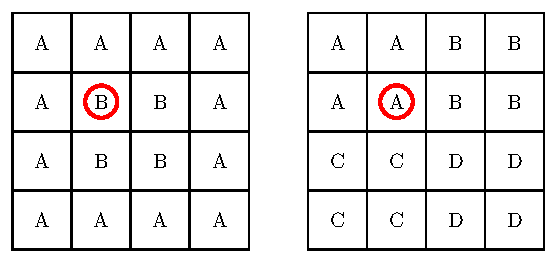
\includegraphics[height=5cm]{target-08-figure-C}
\end{center}
In the second configuration above, color D could also be replaced with color A. And color B and C could be the same. So in effect, we have four possible colorings: 
\begin{center}
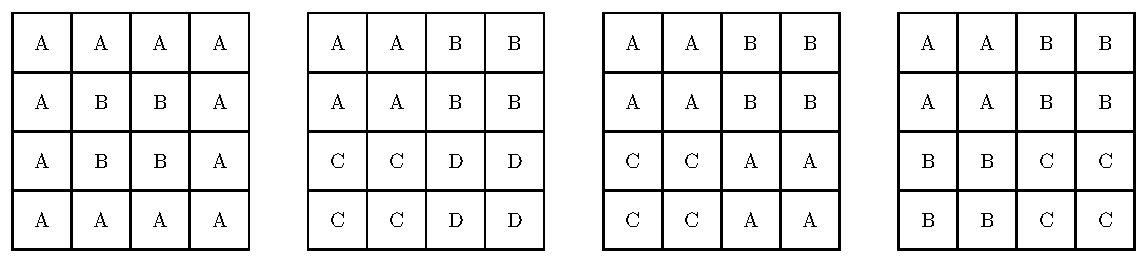
\includegraphics[width=\linewidth]{target-08-figure-D}
\end{center}
Since A, B, C, and D are placeholders for the colors, we now count the permutations for each case. In the first case, there are $4$ choices for color A and thereafter $3$ choices for color B:
\begin{align*}
4 \times 3 = 12 
\end{align*}
In the second case, there are $4$ choices for color A, $3$ choices for B, $2$ choices for C:
\begin{align*}
4 \times 3 \times 2 = 24
\end{align*}
In the third case, there are $4$ choices for color A, $3$ choices for B, and $2$ choices for $C$:
\begin{align*}
4 \times 3 \times 2 = 24
\end{align*}
In the fourth case, there are $4$ choices for color A, $3$ choices for B, and $3$ choices for $C$:
\begin{align*}
4 \times 3 \times 3 = 36
\end{align*}
The total number of colorings is therefore:
\begin{align*}
12 + 24 + 24 + 36 = 96
\end{align*}
\begin{empheq}[box={\mathbox[colback=white]}]{equation*}
    96 ~\text{ways}
\end{empheq} 
\end{answer}
%%%%%%%%%%%%%%%%%%%%%%%%%%%%%%%%%%%%%%%%%%%%%%%%%%%%%%%%%%%%%%%%%%%%%%%%


\end{document}